%%%%%%%%%%%%%%%%%%%%%%%%%%%%%%%%%%%%%%%%%%%%%%%%%%%%%%%%%%%%%%%%%%%%%
%% This is a (brief) model paper using the achemso class
%% The document class accepts keyval options, which should include
%% the target journal and optionally the manuscript type.
%%%%%%%%%%%%%%%%%%%%%%%%%%%%%%%%%%%%%%%%%%%%%%%%%%%%%%%%%%%%%%%%%%%%%
\documentclass[journal=jacsat,manuscript=article]{achemso}

%%%%%%%%%%%%%%%%%%%%%%%%%%%%%%%%%%%%%%%%%%%%%%%%%%%%%%%%%%%%%%%%%%%%%
%% Place any additional packages needed here.  Only include packages
%% which are essential, to avoid problems later. Do NOT use any
%% packages which require e-TeX (for example etoolbox): the e-TeX
%% extensions are not currently available on the ACS conversion
%% servers.
%%%%%%%%%%%%%%%%%%%%%%%%%%%%%%%%%%%%%%%%%%%%%%%%%%%%%%%%%%%%%%%%%%%%%
\usepackage[version=3]{mhchem} % Formula subscripts using \ce{}
\usepackage[T1]{fontenc}       % Use modern font encodings

\usepackage{color}
\usepackage{xr}
\externaldocument{suppinfo}

%%%%%%%%%%%%%%%%%%%%%%%%%%%%%%%%%%%%%%%%%%%%%%%%%%%%%%%%%%%%%%%%%%%%%
%% If issues arise when submitting your manuscript, you may want to
%% un-comment the next line.  This provides information on the
%% version of every file you have used.
%%%%%%%%%%%%%%%%%%%%%%%%%%%%%%%%%%%%%%%%%%%%%%%%%%%%%%%%%%%%%%%%%%%%%
%%\listfiles

%%%%%%%%%%%%%%%%%%%%%%%%%%%%%%%%%%%%%%%%%%%%%%%%%%%%%%%%%%%%%%%%%%%%%
%% Place any additional macros here.  Please use \newcommand* where
%% possible, and avoid layout-changing macros (which are not used
%% when typesetting).
%%%%%%%%%%%%%%%%%%%%%%%%%%%%%%%%%%%%%%%%%%%%%%%%%%%%%%%%%%%%%%%%%%%%%
\newcommand*\mycommand[1]{\texttt{\emph{#1}}}

\newcommand{\cli}{Cl$^{-}$}
\newcommand{\ki}{K$^{+}$}

\newcommand{\tsveta}[1]{\textcolor{red}{#1}}
\newcommand{\nico}[1]{\textcolor{red}{#1}}
\newcommand{\kolya}[1]{\textcolor{blue}{#1}}
\newcommand{\denis}[1]{\textcolor{green}{#1}}

%%%%%%%%%%%%%%%%%%%%%%%%%%%%%%%%%%%%%%%%%%%%%%%%%%%%%%%%%%%%%%%%%%%%%
%% Meta-data block
%% ---------------
%% Each author should be given as a separate \author command.
%%
%% Corresponding authors should have an e-mail given after the author
%% name as an \email command. Phone and fax numbers can be given
%% using \phone and \fax, respectively; this information is optional.
%%
%% The affiliation of authors is given after the authors; each
%% \affiliation command applies to all preceding authors not already
%% assigned an affiliation.
%%
%% The affiliation takes an option argument for the short name.  This
%% will typically be something like "University of Somewhere".
%%
%% The \altaffiliation macro should be used for new address, etc.
%% On the other hand, \alsoaffiliation is used on a per author basis
%% when authors are associated with multiple institutions.
%%%%%%%%%%%%%%%%%%%%%%%%%%%%%%%%%%%%%%%%%%%%%%%%%%%%%%%%%%%%%%%%%%%%%
\author{Tsveta Miteva}
\affiliation{Sorbonne Universit\'{e}s, UPMC Univ Paris 06, UMR 7614, Laboratoire de Chimie Physique Mati\`{e}re et Rayonnement, F-75005 Paris, France}

\author{Nikolai Kryzhevoi}
\affiliation{Theoretische Chemie, Physikalisch-Chemisches Institut, Universit\"at Heidelberg, Im Neuenheimer Feld 229, D-69120 Heidelberg, Germany}

\author{Nicolas Sisourat}
\affiliation{Sorbonne Universit\'{e}s, UPMC Univ Paris 06, UMR 7614, Laboratoire de Chimie Physique Mati\`{e}re et Rayonnement, F-75005 Paris, France}

\author{Ch. Nicolas}
\affiliation{Sorbonne Universit\'{e}s, UPMC Univ Paris 06, UMR 7614, Laboratoire de Chimie Physique Mati\`{e}re et Rayonnement, F-75005 Paris, France}

\author{Wandared Pokapanich}
\affiliation{Sorbonne Universit\'{e}s, UPMC Univ Paris 06, UMR 7614, Laboratoire de Chimie Physique Mati\`{e}re et Rayonnement, F-75005 Paris, France}

\author{Th. Saisopa}
\affiliation{Sorbonne Universit\'{e}s, UPMC Univ Paris 06, UMR 7614, Laboratoire de Chimie Physique Mati\`{e}re et Rayonnement, F-75005 Paris, France}

\author{P. Songsiriritthigul}
\affiliation{Sorbonne Universit\'{e}s, UPMC Univ Paris 06, UMR 7614, Laboratoire de Chimie Physique Mati\`{e}re et Rayonnement, F-75005 Paris, France}

\author{Y. Rattanachai}
\affiliation{Sorbonne Universit\'{e}s, UPMC Univ Paris 06, UMR 7614, Laboratoire de Chimie Physique Mati\`{e}re et Rayonnement, F-75005 Paris, France}

\author{Andreas Dreuw}
\affiliation{Interdisciplinary Center for Scientific Computing, Ruprecht-Karls University, Im Neuenheimer Feld 205A, D-69120 Heidelberg, Germany}

\author{Jan Wenzel}
\affiliation{Interdisciplinary Center for Scientific Computing, Ruprecht-Karls University, Im Neuenheimer Feld 205A, D-69120 Heidelberg, Germany}

\author{Ralph P\"{u}ttner}
\affiliation{Sorbonne Universit\'{e}s, UPMC Univ Paris 06, UMR 7614, Laboratoire de Chimie Physique Mati\`{e}re et Rayonnement, F-75005 Paris, France}

\author{J\'{e}r\^ome Palaudoux}
\affiliation{Sorbonne Universit\'{e}s, UPMC Univ Paris 06, UMR 7614, Laboratoire de Chimie Physique Mati\`{e}re et Rayonnement, F-75005 Paris, France}

\author{Gunnar \"{O}hrwall}
\affiliation{Sorbonne Universit\'{e}s, UPMC Univ Paris 06, UMR 7614, Laboratoire de Chimie Physique Mati\`{e}re et Rayonnement, F-75005 Paris, France}

\author{Lorenz S. Cederbaum}
\affiliation{Theoretische Chemie, Physikalisch-Chemisches Institut, Universit\"at Heidelberg, Im Neuenheimer Feld 229, D-69120 Heidelberg, Germany}

\author{Jean Pascal Rueff}
\affiliation{Sorbonne Universit\'{e}s, UPMC Univ Paris 06, UMR 7614, Laboratoire de Chimie Physique Mati\`{e}re et Rayonnement, F-75005 Paris, France}
\affiliation{Synchrotron SOLEIL, l`Orme des Merisiers, Saint-Aubin, F-91192 Gif-sur-Yvette Cedex, France}

\author{Denis C\'{e}olin}
\email{denis.ceolin@synchrotron-soleil.fr}
\affiliation{Synchrotron SOLEIL, l`Orme des Merisiers, Saint-Aubin, F-91192 Gif-sur-Yvette Cedex, France}

%%%%%%%%%%%%%%%%%%%%%%%%%%%%%%%%%%%%%%%%%%%%%%%%%%%%%%%%%%%%%%%%%%%%%
%% The document title should be given as usual. Some journals require
%% a running title from the author: this should be supplied as an
%% optional argument to \title.
%%%%%%%%%%%%%%%%%%%%%%%%%%%%%%%%%%%%%%%%%%%%%%%%%%%%%%%%%%%%%%%%%%%%%
\title[]
  {The all-seeing eye of resonant Auger electron spectroscopy: a study on aqueous KCl}

%%%%%%%%%%%%%%%%%%%%%%%%%%%%%%%%%%%%%%%%%%%%%%%%%%%%%%%%%%%%%%%%%%%%%
%% Some journals require a list of abbreviations or keywords to be
%% supplied. These should be set up here, and will be printed after
%% the title and author information, if needed.
%%%%%%%%%%%%%%%%%%%%%%%%%%%%%%%%%%%%%%%%%%%%%%%%%%%%%%%%%%%%%%%%%%%%%
\abbreviations{AES,XAS}
\keywords{Solvated ions, resonant Auger spectroscopy, X-ray absorption spectroscopy}

%%%%%%%%%%%%%%%%%%%%%%%%%%%%%%%%%%%%%%%%%%%%%%%%%%%%%%%%%%%%%%%%%%%%%
%% The manuscript does not need to include \maketitle, which is
%% executed automatically.
%%%%%%%%%%%%%%%%%%%%%%%%%%%%%%%%%%%%%%%%%%%%%%%%%%%%%%%%%%%%%%%%%%%%%
\begin{document}

%%%%%%%%%%%%%%%%%%%%%%%%%%%%%%%%%%%%%%%%%%%%%%%%%%%%%%%%%%%%%%%%%%%%%
%% The "tocentry" environment can be used to create an entry for the
%% graphical table of contents. It is given here as some journals
%% require that it is printed as part of the abstract page. It will
%% be automatically moved as appropriate.
%%%%%%%%%%%%%%%%%%%%%%%%%%%%%%%%%%%%%%%%%%%%%%%%%%%%%%%%%%%%%%%%%%%%%
\begin{tocentry}

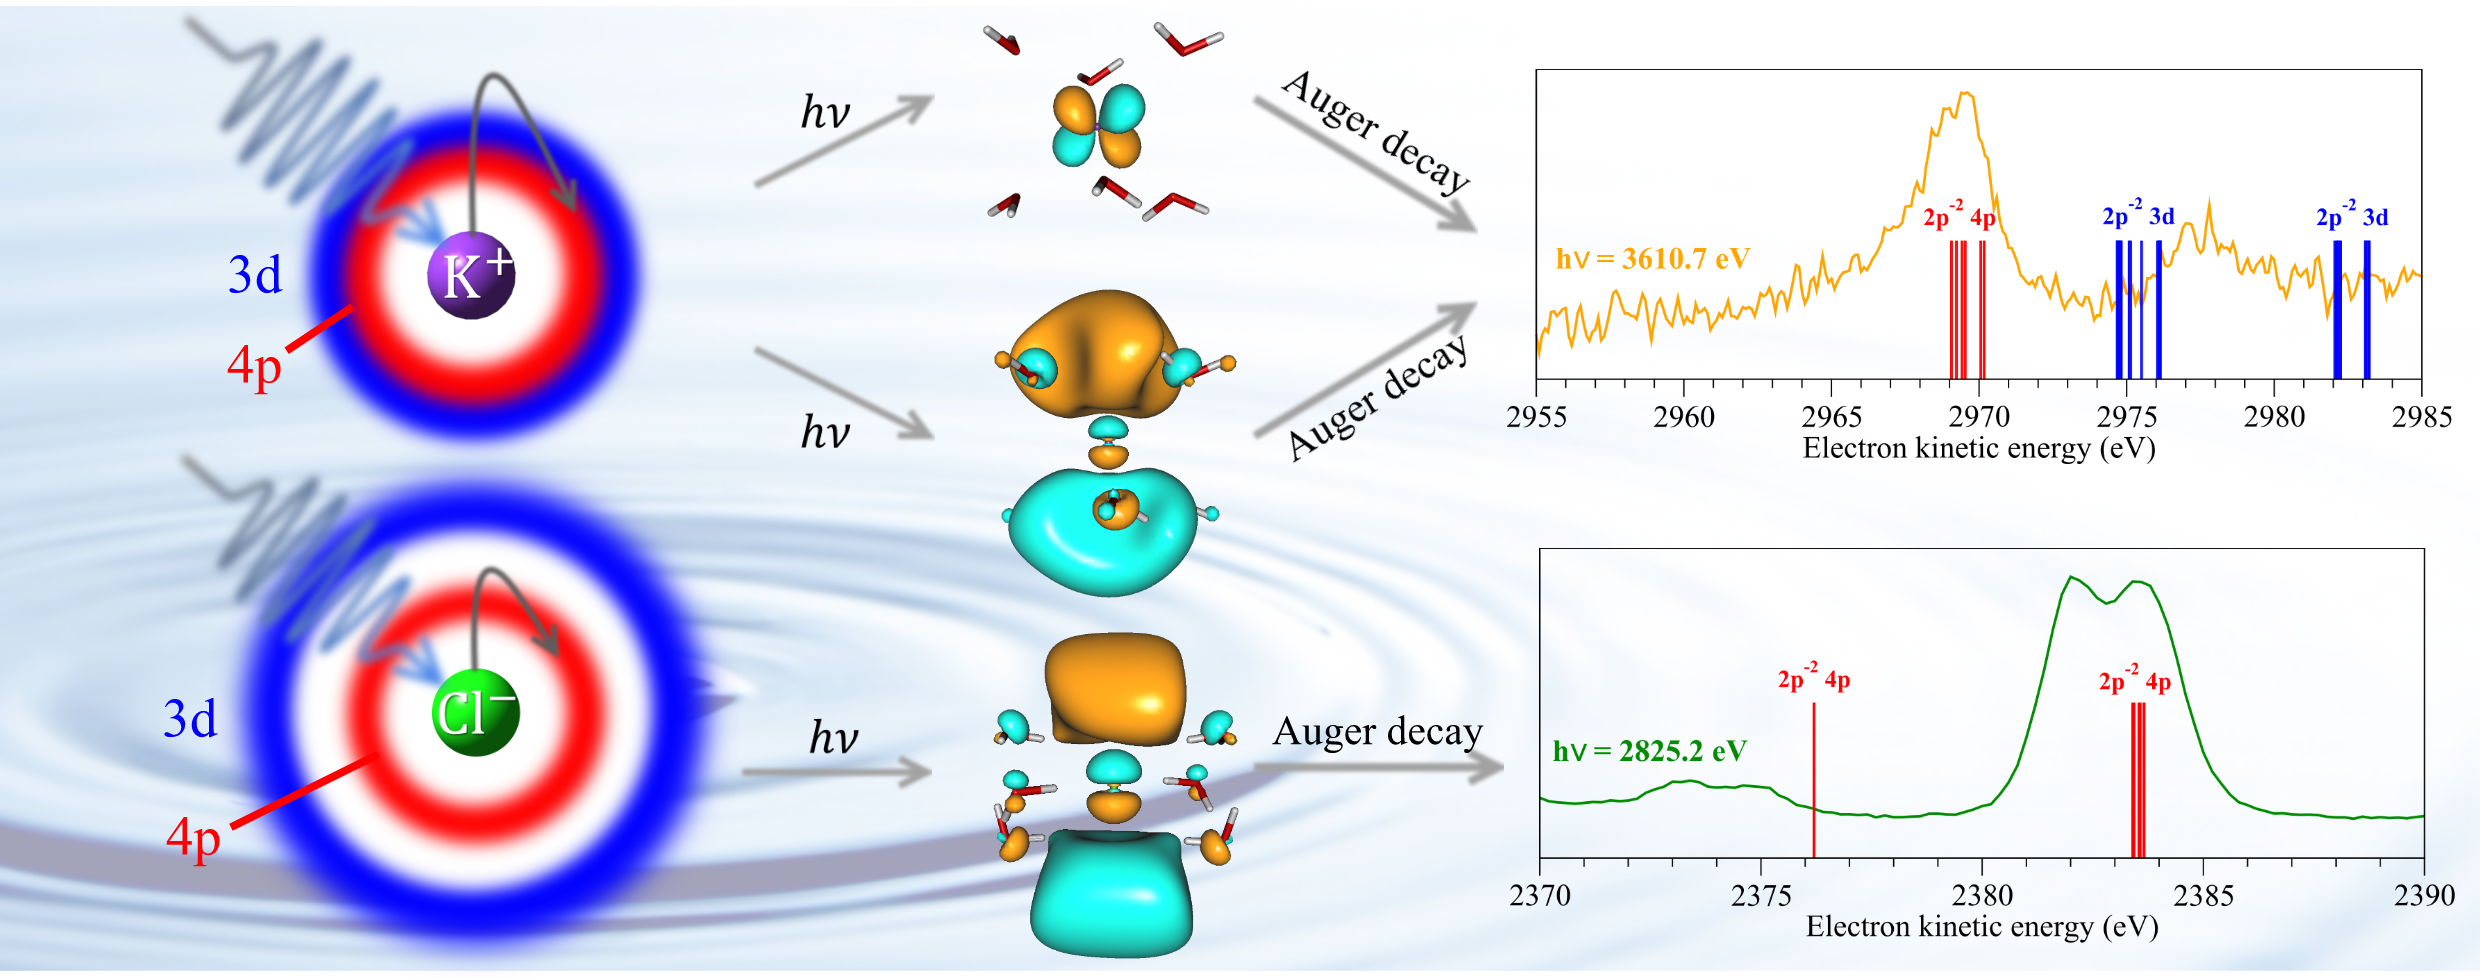
\includegraphics[scale=0.82]{figures/graphical.png}
%Some journals require a graphical entry for the Table of Contents.
%This should be laid out ``print ready'' so that the sizing of the
%text is correct.
%
%Inside the \texttt{tocentry} environment, the font used is Helvetica
%8\,pt, as required by \emph{Journal of the American Chemical
%Society}.
%
%The surrounding frame is 9\,cm by 3.5\,cm, which is the maximum
%permitted for  \emph{Journal of the American Chemical Society}
%graphical table of content entries. The box will not resize if the
%content is too big: instead it will overflow the edge of the box.
%
%This box and the associated title will always be printed on a
%separate page at the end of the document.

\end{tocentry}

%%%%%%%%%%%%%%%%%%%%%%%%%%%%%%%%%%%%%%%%%%%%%%%%%%%%%%%%%%%%%%%%%%%%%
%% The abstract environment will automatically gobble the contents
%% if an abstract is not used by the target journal.
%%%%%%%%%%%%%%%%%%%%%%%%%%%%%%%%%%%%%%%%%%%%%%%%%%%%%%%%%%%%%%%%%%%%%
\begin{abstract}
 X-ray absorption and Auger electron spectroscopies are powerful tools to probe the electronic structure and immediate surroundings of ions in solution. Using these techniques, we study the electronic structure and decay of aqueous KCl at the K-edges of \ki~and \cli. Although the two ions are isoelectronic, their Auger electron spectra exhibit notably different features. This is due to the energetic proximity of the 1s$^{-1}$3d and 1s$^{-1}$4p core excited states in the bare \ki~ion leading to their mixing in the presence of the solvent. As a result, the dipole forbidden 1s$^{-1}$3d state is populated upon K-shell excitation of aqueous K$^{+}$, and its resonant Auger decay of this state results in a separate feature in the Auger electron spectrum of \ki~which is absent in the spectrum of \cli. The results of this work represent a pioneering study of the decay processes initiated by photoabsorption in the tender x-ray regime close to threshold in liquids.


%X-ray absorption and Auger electron spectroscopies are powerful tools to probe the electronic structure and immediate surroundings of ions in solution. In this work we use a combination of these methods together with {\it ab initio} calculations to study the electronic structure and decay in aqueous KCl at the K-edges of \ki~and \cli. Although the two ions are isoelectronic, their Auger electron spectra exhibit notably different features. To explain these differences, we carried out {\it ab initio} calculations of both the core excited states and the final Auger states of bare \ki, \cli~and their microsolvated clusters. This is due to the fact that the energetic order of the 1s$^{-1}$3d and 1s$^{-1}$4p core excited states is inverted in \ki~with respect to \cli, and moreover the two states lie energetically close in the bare \ki~ion leading to their mixing in the presence of the solvent. As a result, the dipole forbidden 1s$^{-1}$3d state is populated upon K-shell excitation of aqueous K$^{+}$. The resonant Auger decay of this state results in a separate feature in the Auger electron spectrum of \ki~which is absent in the spectrum of \cli. The results of this work represent a pioneering study of the decay processes initiated by photoabsorption in the tender x-ray regime close to threshold in liquids and are thus of importance in unveiling the mechanisms of radiation damage in biologically relevant systems.
%Denis: line 2, I replaced spectroscopies by methods
\end{abstract}

%%%%%%%%%%%%%%%%%%%%%%%%%%%%%%%%%%%%%%%%%%%%%%%%%%%%%%%%%%%%%%%%%%%%%
%% Start the main part of the manuscript here.
%%%%%%%%%%%%%%%%%%%%%%%%%%%%%%%%%%%%%%%%%%%%%%%%%%%%%%%%%%%%%%%%%%%%%
\section{Introduction}

X-ray absorption and Auger electron spectroscopies are powerful tools to study the electronic structure and the nearest environment of atoms and molecules in gas, liquid and solid phase. Understanding how atoms or molecules respond to irradiation with x-rays gives insight into the structure of solutions (see Ref.\ \citep{smith17:13909} and references therein), and the mechanism of radiation damage \citep{ONeill02:329,Carugo05:213,Stumpf16:237}. Upon absorption of an x-ray photon, core excited or core ionized states of a specific atom are populated depending on the photon energy. The relaxation of these highly energetic states involves an ultrafast cascade of intraatomic processes, such as radiative and Auger decays. Furthermore, if the initially excited or ionized species is embedded in an environment, interatomic processes such as charge and energy transfer \citep{Pokapanich09:7264,Pokapanich11:13430,Stumpf16:237,unger17:708,ceolin17:263003} are possible.


The course of a decay cascade depends on the character of the initially populated states. This has been well understood in atoms and molecules in gas phase  \citep{stoychev08:074307,Demekhin08:043421,Demekhin09:104303,Ouchi11:053415,Miteva14:164303,travnikova16:213001,Gokhberg14:661,Trinter14:664}. In the case of a core ionized state, the Auger decay process, designated as normal Auger decay (see Fig.\ \ref{fg:auger}), leads to the population of doubly ionized final states localized on the initially ionized unit \citep{stoychev08:074307,Demekhin08:043421,Demekhin09:104303,Ouchi11:053415}. Auger processes in rare gas clusters have been also investigated (refs). The normal Auger decay process in clusters proceeds similarly to that in atoms or molecules. However, in the case of a core excited state, the resonant Auger process competes with the process of delocalization of the excited electron in clusters. If the initially core excited electron delocalizes within the lifetime of the core hole, then normal instead of resonant Auger decay is observed \citep{Bjorneholm95:3017}. 

%refs clusters??:
%A. Lindblad, R. F. Fink, H. Bergersen, M. Lundwall, T. Rander, R. Feifel, G. Öhrwall, M. Tchaplyguine, U.Hergenhahn, S. Svensson, O. Björneholm, The Journal of Chemical %Physics 123, 211101 (2005)
%M. Tchaplyguine, A. Kivimäki, S. Peredkov, S. L. Sorensen, G. Öhrwall, J. Schulz, M. Lundwall, T. Rander, A. Lindblad, A. Rosso, S. Svensson, N. Mårtensson, O. %Björneholm, The Journal of Chemical Physics, 127, 124314 (2007)


In a solution, the electronic decay processes initiated by x-ray photoabsorption are different compared to those in rare gas clusters due to the shorter distances and stronger interatomic interactions. In particular, the solvent molecules have two effects -- first, they strongly affect the excited \citep{miteva16:16671} or ionized states of the ion and second, they can participate in the decay processes, leading to the population of charge-separated final states, and ionization of the surrounding environment \citep{Pokapanich09:7264,Pokapanich11:13430,Stumpf16:237,ceolin17:263003}. Moreover, the process of delocalization of the initially excited electron also occurs in aqueous solutions \citep{Nordlund07:217406,Ottosson11:13489}.
%Moreover, the process of delocalization of the initially excited electron is not specific to rare gas clusters, but it also occurs in aqueous solutions \citep{Nordlund07:217406,Ottosson11:13489}. 
In the case of pure water, the rate of delocalization of the O1s excited electron takes place on a femtosecond to sub-femtosecond time scale depending on the photon energy, thus being commensurate with the lifetime of the O1s core hole which is 6\,fs \citep{Nordlund07:217406}. The O K-edge is located in the soft x-ray range of photon energies. Going higher in photon energy, in the tender and hard x-ray regimes, the lifetimes of the core ionized or core excited states become even shorter, on the order of 1\,fs. And thus, it is even more imperative to reveal whether the delocalization of the core excited electron occurs within the lifetime of the core hole.


The aim of this work is to elucidate the nature of the states populated upon x-ray irradiation of solvated ions in the tender x-ray regime, and furthermore, to understand whether the process of delocalization influences the resonant Auger decay. To this end, we used Auger electron spectroscopy together with x-ray absorption spectroscopy in the tender x-ray regime to study aqueous potassium chloride at the K-edges of both \ki~and \cli. In particular, we demonstrate experimentally that at photon energies below the K-edges of the two ions, localized core excited states are populated. These states undergo resonant Auger decay within less than 1\,fs. In both ions, there is a competition between resonant Auger decay and delocalization of the excited electron. Using the core-hole clock method we show that in \ki~delocalization at the pre-edge is weak, whereas in the case of \cli, due to the energetic proximity of the core excited state to the K-edge, the rate of delocalization is of the same order as that of the resonant Auger process. Moreover, we observe that although the \ki~and \cli~ions are isoelectronic, they have different fingerprints in the resonant Auger spectra. With the aid of high-level {\it ab initio} calculations of the initial and final states of the resonant Auger process of both the bare ions and their microsolvated clusters, we demonstrate that these differences result from different electronic structures of the two ions, thus confirming that the combination of XAS and AES techniques is a sensitive probe of the electronic structure of solutions.


\begin{figure}
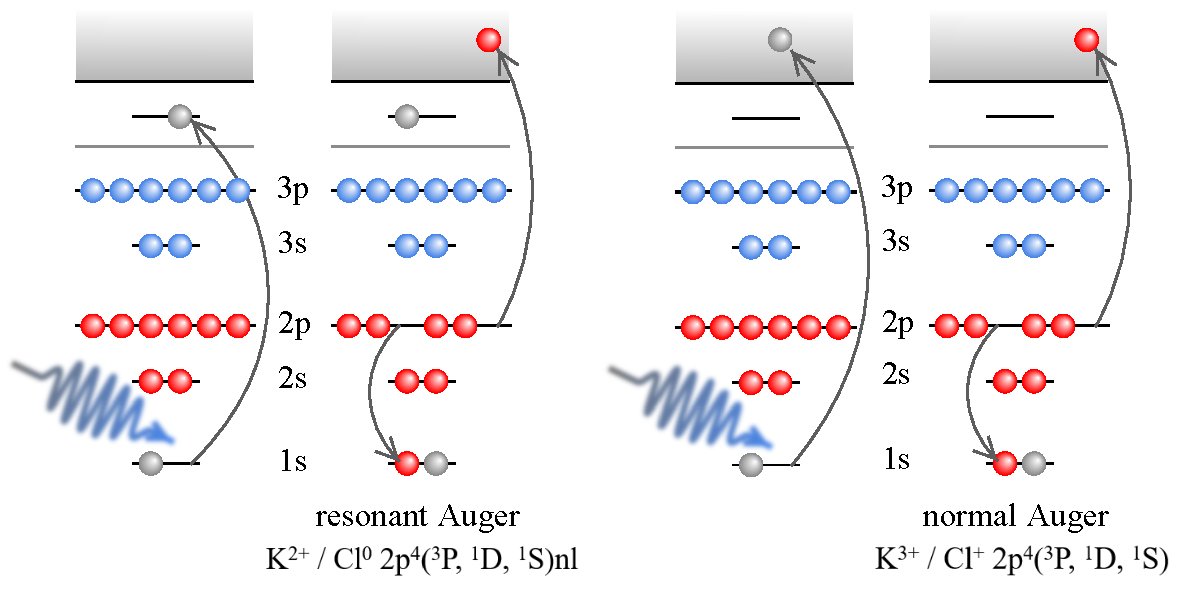
\includegraphics[scale=0.8]{figures/auger_process.pdf}
\caption{Schematic representation of the normal and resonant Auger processes of the isoelectronic \ki~and \cli~ions. The charges of the final Auger states in the two ions are also shown.}
\label{fg:auger}
\end{figure}

\section{Methods} \label{sec:methods}
\subsection{Experimental}
% Denis, please have a look at the experimental part and see if all the references have been correctly included

For the present experiment we used the newly operational microjet setup that was specifically designed for the HAXPES station of the GALAXIES beamline, in collaboration with the Microliquids Company. Details of the beamline are given in the reference [JPR] and details on the electron spectrometer are given in the reference \citep{ceolin15:022502,ceolin13:188}. Due to the limited amount of space available if front of the analyzer lens and due to the limited number of ports available on the main vacuum chamber, the challenge was to arrange all the elements composing the microjet setup in a very compact manner. A differentially-pumped tube in which the microjet assembly is inserted, is installed in front of the spectrometer lens and can be moved independently from the main vacuum chamber by means of a three axes motorized manipulator. Two holes of 2 mm diameter allow the photons to go in and out of the tube, and a third one, on which is mounted a skimmer having a 500$\mu$m diameter hole, allows the electrons created at the interaction point to go in the direction of the spectrometer lens. To ensure a proper vacuum in the differentially pumped tube, a 5-way cross is connected to it and holds a 1200 l/s turbo pump, a liquid nitrogen trap, a vacuum gage and the liquid/electrical feedthroughs. A rail, fixed at the bottom of the tube, is used to slides precisely an insert on which the different elements necessary for the injection, control, collection and visualization of the liquid are mounted.


The head of this insert is mostly composed by: a glass capillary fixed by a dedicated peek-piece, a catcher in CuBe with a 300$\mu$m hole, a piezo motors stage allowing a precise control of these last two parts, and a camera. The catcher is placed at a distance of about 5mm from the capillary and is permanently pumped in order to extract the liquid from the vacuum chamber. For the present experiment, a 0.5M KCl aqueous solution is injected in a capillary having a 30$\mu$m diameter, by a HPLC pump with a constant flux of 1.6 ml/min. The catcher temperature is controlled so that the liquid does not freeze before its extraction. Considering that the photon propagation axis, the spectrometer lens axis and the liquid microjet form an orthogonal trihedron, the piezo motorization allows moving the liquid microjet along the photon propagation and the lens axes during the experiment if necessary. The catcher can be moved by the piezo motors along the photon propagation axis only. A simple camera is used to control the liquid jet positioning as compared with the catcher hole. The alignment of the full head (particularly capillary plus catcher) as compared with the X-ray beam is performed by moving the whole system using the 3-axes motorized manipulator. The alignment of the setup is performed by measuring the O1s XPS peak intensity of a simple salt aqueous solution, and by optimizing the liquid phase vs gas phase ratio. The pressure in the main chamber was kept below the 10$^{-5}$ mbar range whereas it was kept at about 10$^{-4}$ mbar in the differentially pumped tube when the HPLC pump was ON. Our equipment is an updated version of the equipment used in the references [3-5]. The aqueous potassium chloride solution was prepared by mixing >99\% KCl salt with deionized water. Filtering and degazing procedures were systematically performed before injecting the solution into the microjet by the HPLC pump.


\subsection{{\bf{\it Ab initio}} calculations}

The X-ray absorption spectra of the microsolvated clusters of potassium and chlorine were computed at the ground state equilibrium geometries of K$^+$(H$_2$O)$_6$ and \cli(H$_2$O)$_6$, which can be considered as representatives of the complete first solvation shell of the two ions \citep{Ohtaki93:1157,soper06:180,ma14:1006}. The two structures were optimized at the DFT level of theory using the B3LYP functional and the 6-311++G(2d,2p) basis set \citep{Krishnan80:650,Blaudeau97:5016}. A frequency analysis was carried out in order to confirm that the obtained geometries are minima on the respective potential energy surfaces. The geometry optimization and frequency analysis were performed with the Gaussian 09 package \citep{g09}. In the case of K$^{+}$(H$_2$O)$_6$ the ground state geometry was obtained by constrained geometry optimization starting with the equilibrium geometry \citep{lee99:3995} belonging to the D$_3$ point group and increasing the angle $\theta$ between the K-O bond and the $C_3$ axis to 55$^{\circ}$. This angle was chosen to be around the maximum in the O-K-O angular distribution obtained from quantum mechanics / molecular mechanics dynamical simulations in Ref.\ \citep{ma14:1006}. {\color{red} the maximum is at 70$^{\circ}$, in our calculation the angle is 90$^{\circ}$} The optimized K-O and Cl-O distances are 2.842~\AA~and 3.333~\AA, respectively, which is in good agreement with other theoretical and experimental works \citep{ge13:13169,gora00:7,Ohtaki93:1157,soper06:180,ma14:1006}. The ground state equilibrium structures are presented in Fig.\ \ref{fg:xas_kcl}. In both cases, they belong D$_3$ point group \citep{rao08:12944,ge13:13169}. 


The energies and transition moments of the core excited states of the microsolvated clusters were computed with the algebraic diagrammatic construction method for the polarization propagator \citep{sch82:2395} within the core-valence separation approximation \citep{bar85:867,ced80:206,ced81:1038} (CVS-ADC(2)x) as implemented in the Q-Chem package \citep{Wenzel14:1900,Wenzel14:4583,Wormit14:774,QChem2015}. In the case of \cli, the 6-311++G(3df,3pd) basis set \citep{Krishnan80:650,McLean80:5639} (excluding the f functions) was used on all atoms, whereas in the case of \ki, we used the 6-311+G(2d,p) basis set \citep{Krishnan80:650,Blaudeau97:5016} on all atoms, and an additional set of 2s, 2p and 2d diffuse functions was added on K. In our calculations, the core space comprises the 1s orbital of K$^{+}$ or \cli, whereas the remaining occupied orbitals are included in the valence space. For the calculations of the XAS spectra we used the C$_2$ point group in the case of K$^{+}$(H$_2$O)$_6$ and \cli(H$_2$O)$_6$. To account for the lifetime broadening due to the Auger decay of the core excited states, we convolved the theoretical spectra with a Lorentzian of FWHM 0.74\,eV and 0.62\,eV in the case of \ki~and \cli, respectively \citep{Krause79:329}. We analyzed the core excited states by expanding the singly occupied natural orbitals (SONOs) $\psi_{i}$ of the microsolvated clusters in the basis of SONOs of the bare K$^{+}$ or \cli~ion $\chi_{nl}$
%
\begin{equation}\label{eq:sono_proj}
\psi_{i} = \sum_{nl} a^{i}_{nl} \chi_{nl}
\end{equation}
%
where $n$ and $l$ stand for the principal and orbital quantum numbers as described in Ref.\ \citep{miteva16:16671}. The expansion coefficients $a^{i}_{nl}$ show the degree of delocalization of the excited electron and the mixing of the core excited states in the crystal field created by the surrounding water molecules (see Fig.\ \ref{fg:xas_kcl}).


The final states following KLL resonant Auger decay of K$^{+}$ and \cli~were computed at the Configuration Interaction Singles (CIS) level using the Graphical Unitary Group Approach (GUGA) as implemented in the GAMESS-US package \citep{GUGA_PhysScr_21,GUGA_JCP_70,GUS}. In order to account for the relaxation effects upon core ionization, we used a restricted open-shell Hartree-Fock reference wave function with a hole in the 2s orbital of both \ki~and \cli.  We used the 6-311++G(2d,2p) basis set \citep{Blaudeau97:5016} augmented with 2s, 2p, 2d diffuse functions on \ki, and the cc-pVTZ basis set augmented with 6s, 6p, 6d diffuse KBJ functions \citep{Kaufmann89:2223} on \cli. The active space comprises the 2s and 2p orbitals of K/Cl with occupancy fixed to 6 and all virtual orbitals with occupancy fixed to 1. The remaining doubly occupied orbitals were frozen in the calculation. \citep{mosnier16:061401}

\section{Results and discussion}\label{sec:rnd}

\begin{figure}%[h]
\centering
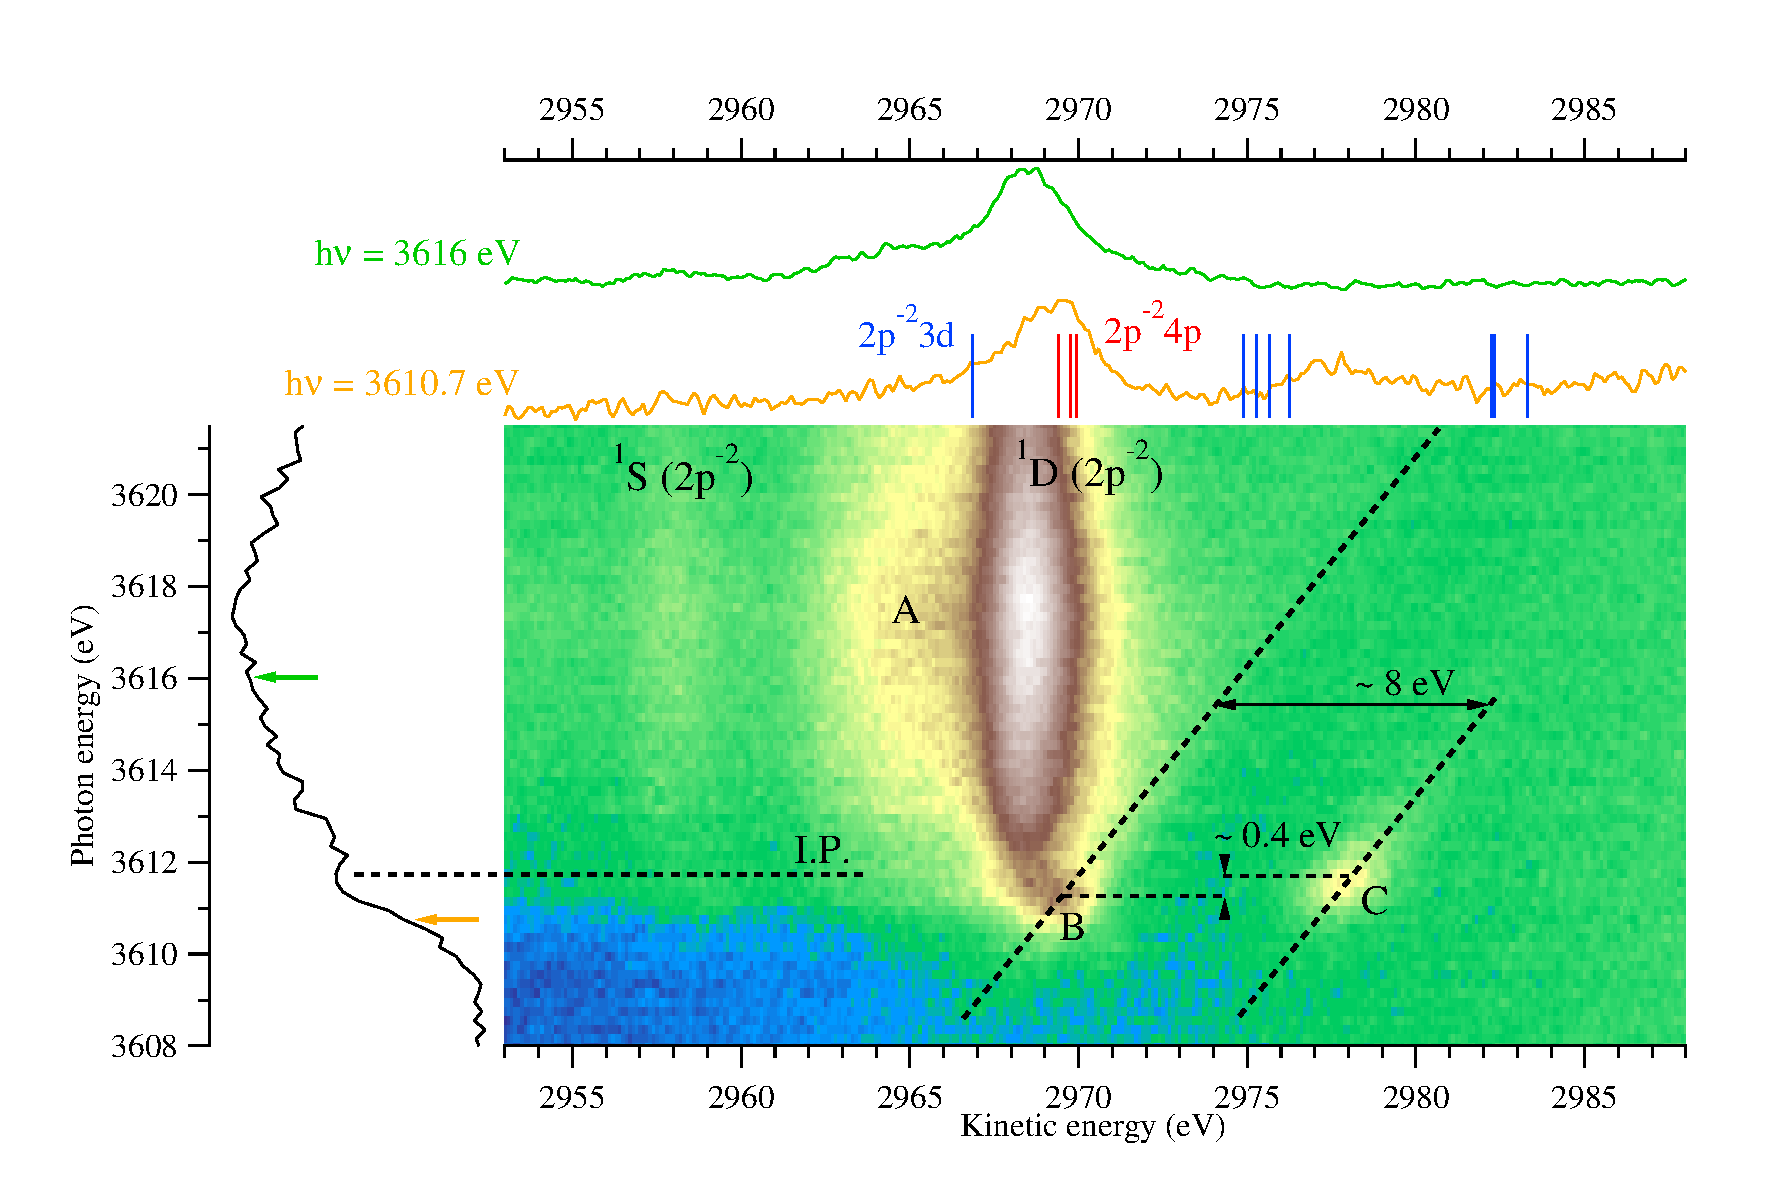
\includegraphics[scale=0.55]{figures/k_2dmap.pdf}
\caption{2D map showing the kinetic energy of the electrons emitted in KL$_{2,3}$L$_{2,3}$ Auger decay vs the photon energy in the vicinity of the K-edge of aqueous K$^{+}$. The black curve on the left represents the experimental partial electron yield spectrum of K$^{+}$ obtained after integrating over the kinetic energies of the Auger electrons in the energy range presented on the figure. The upper panel shows two spectra at photon energies 3610.7\,eV, and 3616\,eV below and above the ionization potential at 3611.9\,eV, respectively. The bars in the pre-edge cut correspond to the final 2p$^{-2}$ 3d (blue) and 2p$^{-2}$4p(red) doublet resonant Auger states of K$^{+}$ computed at the CIS level (see Sec.\ \ref{sec:methods} for details). The features A, B and C are discussed in the text.}
\label{fg:2dmap_k}
\end{figure}


\begin{figure}%[h]
\centering
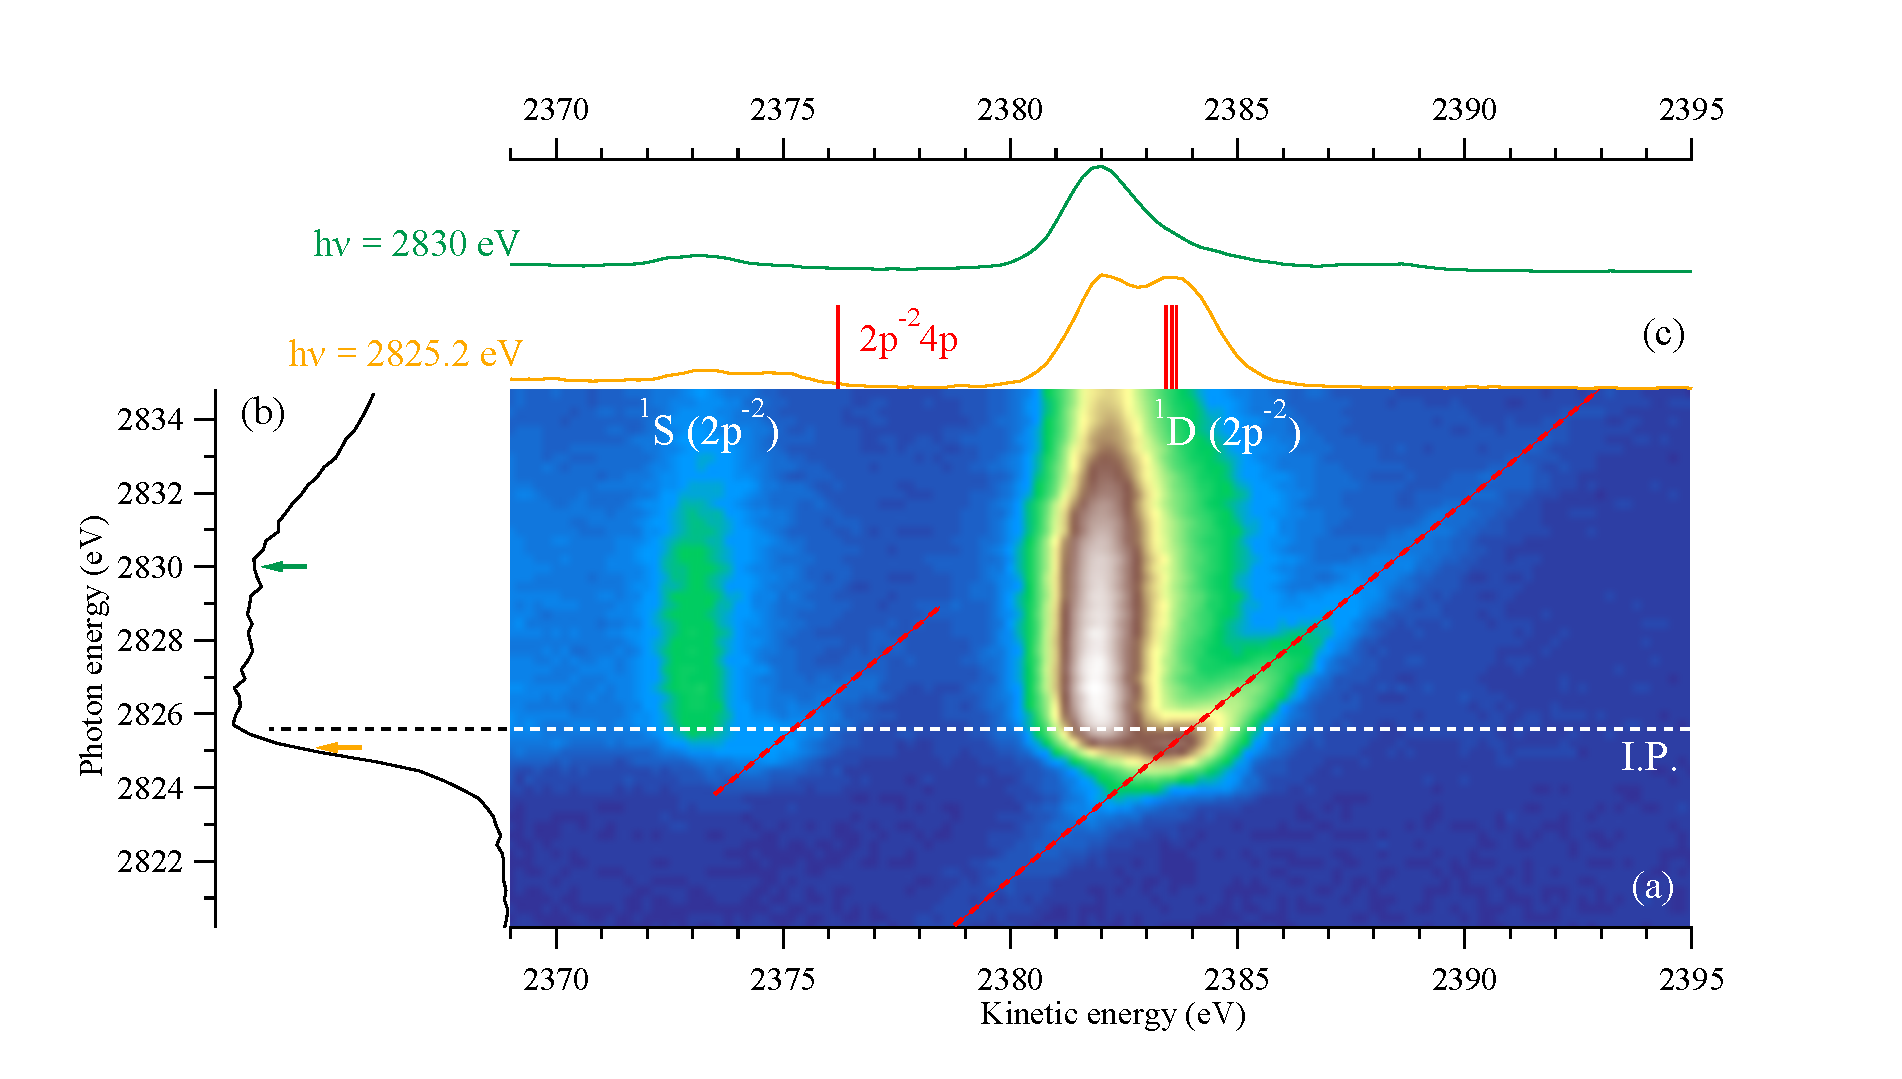
\includegraphics[scale=0.55]{figures/cl_2dmap.pdf}
\caption{2D map showing the kinetic energy of the electrons emitted in KL$_{2,3}$L$_{2,3}$ Auger decay vs the photon energy in the vicinity of the K-edge of aqueous Cl$^{-}$. The black curve on the left represents the experimental partial electron yield spectrum of Cl$^{-}$ obtained after integrating over the kinetic energies of the Auger electrons in the energy range presented on the figure. The upper panel shows two spectra at photon energies 2825.2\,eV, and 2830.0\,eV below and above the ionization potential at 2825.4\,eV, respectively. The bars in the pre-edge cut correspond to the final 2p$^{-2}$ 3d (blue) and 2p$^{-2}$4p(red) doublet resonant Auger states of K$^{+}$ computed at the CIS level (see Sec.\ \ref{sec:methods} for details).}
\label{fg:2dmap_cl}
\end{figure}


\subsection{Normal Auger decay}\label{ssec:na}

The KL$_{2,3}$L$_{2,3}$ normal Auger decay following K-shell ionization of aqueous \ki~and \cli~can be written as follows
%
\begin{align*}
\gamma + \text{K}^{+}_{\text{aq}} \rightarrow \text{K}^{2+}_{\text{aq}} (1s^{-1}) \rightarrow \text{K}^{3+}_{\text{aq}} (2p^{-2}) + e^{-}_{\text{Auger}}\\
\gamma + \text{Cl}^{-}_{\text{aq}} \rightarrow \text{Cl}^{0}_{\text{aq}} (1s^{-1}) \rightarrow \text{Cl}^{+}_{\text{aq}}(2p^{-2}) + e^{-}_{\text{Auger}}
\end{align*}
%
It results in the population of 2p$^{-2}$($^3$P, $^1$D, $^1$S) final states. The $^3$P final states are not observed in the experiment since they are forbidden from parity conservation rules. In the case of Cl$^{-}_{\text{aq}}$, the lines corresponding to the Cl$^{+}$ (2p$^{-2}$) $^1$S and $^1$D states are located at 2373.2\,eV and 2382.1\,eV kinetic energy (see Fig.\ \ref{fg:2dmap_cl}). For K$^{+}_{\text{aq}}$ the maxima of the $^1$S and $^1$D KL$_{2,3}$L$_{2,3}$ Auger lines are located at 2958\,eV and 2968.4\,eV, respectively (see Fig.\ \ref{fg:2dmap_k}). 


The KL$_{2,3}$L$_{2,3}$ Auger lines do not disperse with photon energy except close to threshold due to the interaction between the photoelectron and Auger electron, i.e.\ the so-called post-collision interaction (PCI). As a result of this interaction, first, the peaks in the Auger spectrum become asymmetric with a shoulder at high kinetic energies, and second, they are shifted to higher kinetic energies close to threshold \citep{russek86:911,guillemin15:012503}. Consequently, one can attribute the high kinetic energy shoulder of the $^1$D and $^1$S peaks on Figs.\ \ref{fg:2dmap_k} and \ref{fg:2dmap_cl} as resulting from PCI effect. In order to quantify this effect we recorded the KLL Auger spectrum of both Cl$^{-}_{\text{aq}}$ and K$^{+}_{\text{aq}}$ at higher photon energies, $h\nu = 5$\,keV (see Ref.\ \citep{ceolin17:263003} for details). In this case, the maxima of the $^1$D and $^1$S states were found at 2381.1\,eV and 2372.3\,eV for Cl$^{-}_{\text{aq}}$, and 2967.4\,eV and 2957\,eV kinetic energy for K$^{+}_{\text{aq}}$, respectively. The lines observed at photon energies far from threshold and close to it appear to be shifted by $\sim$1\,eV. The magnitude of the shift is the same for both ions suggesting that it does not depend on the initial charge of the ion. The observed PCI shift of 1\,eV is larger than in the case of the isoelectronic Ar, where its value is $\sim$0.5\,eV at a photon energy of 10 \,eV above threshold \citep{guillemin15:012503}. The shift in the energies of the photo- and Auger electrons is proportional to the change in the ionic field during the Auger process. In a solution, both the single and double ionization potentials change due to the polarization of the water molecules and the stabilization of the ionic species through ion-dipole interaction with the polarized solvent. For example, in \ki, the ionization potential of the bare ion was experimentally determined to be 3619.4\,eV \citep{hertlein06:062715}, whereas in an aqueous solution, its value drops by about 7.5\,eV. The magnitude of this effect increases with the ionic charge, consequently, there will be an even greater difference for the double ionization potential. Thus, one can expect a larger change in the ionic field in an aqueous solution compared to that in a van der Waals cluster, which can, therefore, account for the large PCI shift of the Auger lines in a solution.


The normal Auger $^1$D main line of K$^{+}$ differs from that of Cl$^{-}$ by the presence of a large shoulder (A on Fig.\ \ref{fg:2dmap_k}) on the low kinetic energy side at about 2965\,eV kinetic energy. This shoulder is attributed to electron transfer from the solvent molecules \citep{ceolin17:263003}. In the case of \cli, there is no experimental evidence of such electron transfer processes.


\subsection{Resonant Auger decay} \label{ssec:ra}

\kolya{XAS of Cl- and K+ from previous works?}

The KL$_{2,3}$L$_{2,3}$ Auger decay following resonant K-shell excitation of solvated \ki~and \cli~can be written as follows
%
\begin{align*}
\gamma + \text{K}^{+}_{\text{aq}} \rightarrow \text{K}^{+*}_{\text{aq}} (1s^{-1}V) \rightarrow \text{K}^{2+}_{\text{aq}} (2p^{-2}V') + e^{-}_{\text{Auger}}\\
\gamma + \text{Cl}^{-}_{\text{aq}} \rightarrow \text{Cl}^{-*}_{\text{aq}} (1s^{-1}V) \rightarrow \text{Cl}^{0}_{\text{aq}}(2p^{-2}V') + e^{-}_{\text{Auger}}
\end{align*}
%
where $V$ and $V'$ denote the virtual orbitals in the excited and singly ionized excited states, i.\ e.\ in the presence of the $1s^{-1}$ and $2p^{-2}$ core holes. The character of these states will be discussed below.


The pre-edge regions of the x-ray absorption spectra of \ki~and \cli~shown to the left on Figs.\ \ref{fg:2dmap_k} and \ref{fg:2dmap_cl} do not exhibit any high intensity features due to the lifetime broadening and energetic proximity of the core excited states to the ionization threshold. Consequently, solely from these spectra, one cannot conclude whether there are core excited states in the pre-edge structure, which can undergo resonant Auger decay. However, one can determine their excitation energies from the maxima of the resonant Auger features. Thus, for \cli, the lowest core excited state is located at 2825.2\,eV, which agrees very well with the position of the Cl$^{-}$ 1s$\,\rightarrow\,$4p excitation determined from Cl K-edge XAS experiments in MgCl$_2$.6H$_2$O and of SrCl$_2$/SrCl$_2$.6H$_2$O \citep{sugiura82:681} and MCl$_{4}^{-}$ compounds \citep{shadle95:2259}. In the case of \ki, there are two dispersive features with maxima at photon energies of 3611.2\,eV (B) and 3611.6\,eV (C), respectively (Fig.\ \ref{fg:2dmap_k}). The positions of these two core excited states are close to the energy of the 1s$\,\rightarrow\,$4p excitation in bare \ki, 3610.7\,eV \citep{hertlein06:062715}.


%Unlike the normal Auger decay, which proceeds in a fairly similar way in the two ions, 
The resonant Auger features produced in the decay of these core excited states appear to be quite different for \cli~and \ki. In the spectrum of \cli~shown in Fig.\ \ref{fg:2dmap_cl} there are two dispersive features on the high kinetic energy side of the main $^1$S and $^1$D lines, i.e.\ at 2825.2\,eV photon energy and 2374.6 and 2383.4\,eV kinetic energy. In the case of \ki, the $^1$S dispersive line cannot be clearly identified due to the presence of strong background. The dispersive feature close to the $^1$D main peak is observed (feature B) with a maximum located at $h\nu = $3611.2 \,eV and 2969.2 \,eV kinetic energy. An additional feature appears as a separate island away from the main lines on the 2D map of \ki. It is located at $h\nu = $3611.6\,eV and 2978.1\,eV kinetic energy (feature C), thus it is separated by approximately 400\,meV photon energy and 8.3\,eV kinetic energy from the feature B. 
%Unlike in the case Cl$^{-}$ the dispersive feature close to the $^1$S main line is not observed in K$^{+}$ due to presence of a strong {\color{red}background (@DENIS?)}. 


%In order to get a better understanding of these features, we will first consider the Auger spectrum of the isoelectronic Ar presented in Refs.\ \citep{ceolin15:022502,guillemin15:012503}. 

%First, from the 2D map of Ar one can extract information about the nature of the core excited states below threshold. The pre-edge structure in the XAS spectrum of Ar consists of the 1s$\,\rightarrow\,$4p and 1s$\,\rightarrow\,$5p excitations. Higher core excited states cannot be identified in the XAS spectrum due to their lifetime broadening and proximity to the ionization threshold. The same excitations were observed in the XAS spectrum of bare \ki~ions \citep{hertlein06:062715}. Again, the identification of 1s$\,\rightarrow\,$np states with n$\,>\,$5 was not possible in the case of \ki.

%Second, the 2D map of Ar carries information about the states populated in the resonant Auger processes following core excitation. In the case of Ar, the Ar 1s$\,\rightarrow\,$4p and 1s$\,\rightarrow\,$5p core excited states undergo both pure spectator and shake-up resonant Auger decay leading to the population of Ar$^{2+}$(2p$^{-2}$np) (n$ = 4 - 6$) final states. As a result, apart from the main Ar$^{2+}(2p^{-2})$ $^1$D and $^1$S lines which result from normal Auger decay, additional dispersive features are observed. For example, the 1s$\,\rightarrow\,$4p core excited state undergoes both pure spectator and shake-up resonant Auger decay. The former results in an island shifted with respect to the main $^1$D line by $\sim$4-5\,eV kinetic energy, whereas the fingerprint of the shake-up process is a feature appearing at the same kinetic energy as the  main $^1$D line. Moreover, the intensities of the observed shake-up features are lower compared to those of the pure spectator Auger decay. In aqueous solutions, one can expect the 2D map to be fairly different as both the initial core excited states and the final Auger states will be influenced by the presence of the solvent.



\begin{figure}[h]
\centering
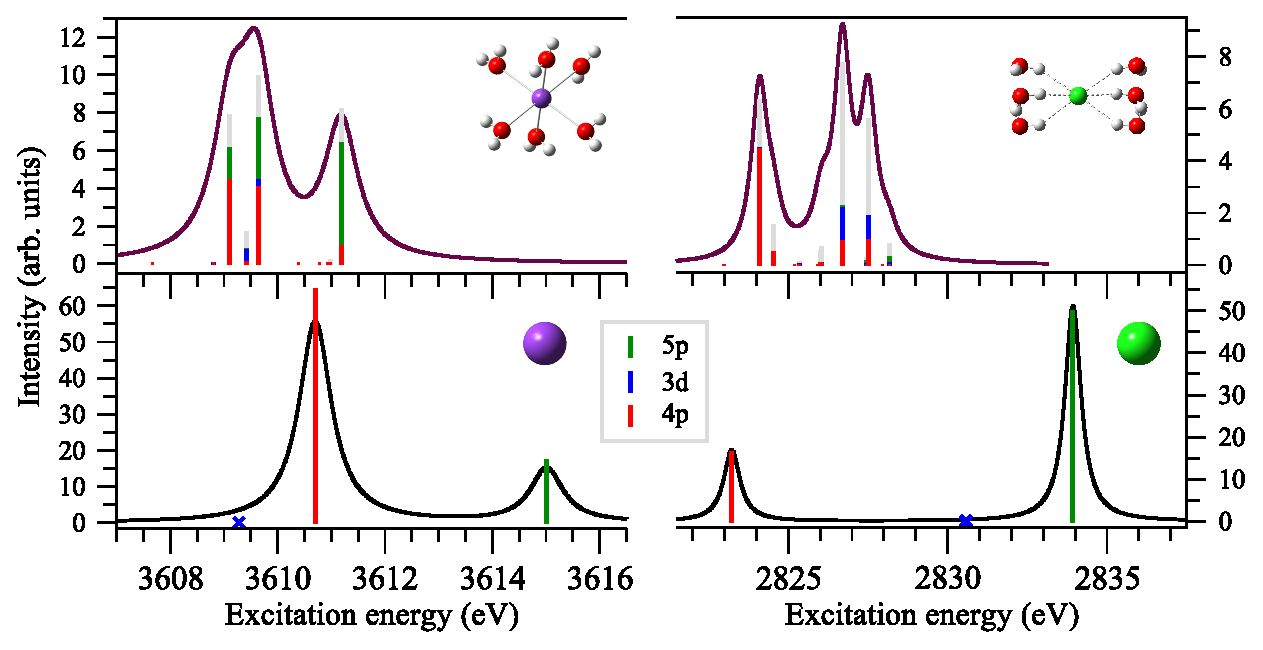
\includegraphics[scale=0.6]{figures/xas_spectra.eps}
\caption{
XAS spectra of the lowest K-shell transitions in the bare K$^{+}$ (lower left panel) and Cl$^{-}$ (lower right panel) ions and their 6-coordinated clusters (upper left panel, \ki(H$_2$O)$_6$, and upper right panel, \cli(H$_2$O)$_6$). The theoretical stick spectra were convolved with a Lorentzian profile of FWHM 0.74\,eV for \ki~and 0.62\,eV for \cli~(dashed line) and a Voigt profile to account for the lifetime broadening and the experimental resolution. The stick spectrum corresponds to the projections $|a_{nl}^{i}|^2$ of the SONOs corresponding to the core excited states of the 6-coordinated clusters on the basis of SONOs corresponding to the 1s$\,\rightarrow\,$3d, 1s$\,\rightarrow\,$4p, and 1s$\,\rightarrow\,$5p states in the bare K$^+$ and \cli~ions (Eq.\ \ref{eq:sono_proj}). The theoretical XAS spectra of both \ki~and \cli~were shifted to higher photon energies such that the excitation energies lowest core excited states correspond to the experimentally determined energies -- 3610.7\,eV in the case of \ki, and 2825.2\,eV in the case of \cli. The experimental ionization thresholds are depicted as grey boxes starting at photon energies of 3611.9\,eV (\ki$_{\text{aq}}$) and 2825.4\,eV (\cli$_{\text{aq}}$).}
\label{fg:xas_kcl}
\end{figure}


In order to rationalize the pre-edge region of the experimental XAS spectra and the differences in the AES spectra of \ki$_{\text{aq}}$ and \cli$_{\text{aq}}$, we computed the lowest core excited states of the bare \ki~and \cli~ions and their hexa-coordinated clusters. The theoretical XAS spectra are presented in Fig.\ \ref{fg:xas_kcl}. In the bare ions (lowermost panels on Fig.\ \ref{fg:xas_kcl}), the lowest energy peak corresponds to the dipole allowed 1s$\,\rightarrow\,$4p state. The next dipole allowed state, 1s$\,\rightarrow\,$5p, is located 4.3\,eV and 10.8\,eV higher in the cases of \ki~and \cli, respectively. Together with the two dipole allowed transitions, we show the dipole forbidden 1s$\,\rightarrow\,$3d states of the bare ions as blue crosses at photon energies 3611.17\,eV in the case of \ki~and 2831.68\,eV in the case of \cli, respectively. It is noteworthy that the positions of the 1s$\,\rightarrow\,$4p and 1s$\,\rightarrow\,$3d states are inverted in \ki~and \cli. In the case of Cl$^{-}$ the 1s$\,\rightarrow\,$4p excitation has lower energy and the 1s$\,\rightarrow\,$3d excitation is close to the 1s$\,\rightarrow\,$5p state. On the contrary, in K$^{+}$ the 1s$\,\rightarrow\,$3d excitation has lower energy and lies below the 1s$\,\rightarrow\,$4p state. We note in passing that the intensity of the Cl$^{-}$(1s$\,\rightarrow\,$4p) state is lower than that of the \cli(1s$\,\rightarrow\,$5p) state contrary to what is observed in \ki. This difference can be explained with the lower electron density of the 4p compared to the 5p electron in the region close to the core hole which thus results in the lower oscillator strength of the 1s$\,\rightarrow\,$4p compared to the 1s$\,\rightarrow\,$5p transition in \cli~(see Fig.\ \ref{fg:rdens_ions}).


The water molecules in the first solvation shell have several effects on the core excited states. First, upon addition of water molecules, the degeneracy of the 1s$\,\rightarrow\,$4p state is lifted and the intensity of the resulting states in the cluster drops. Moreover, the character of these states changes -- they are no longer of pure atomic character but they rather interact with states of the neighboring water molecules (shown as grey bars) and with other closely lying states of the bare ion, such as the dipole allowed 1s$\,\rightarrow\,$5p and dipole forbidden 1s$\,\rightarrow\,$3d state. Thus, the latter also acquire intensity in the cluster due to mixing with the dipole allowed states in the ligand field of the solvent. A similar effect was observed in the XAS spectra of microsolvated clusters of Na$^{+}$ and Mg$^{2+}$ \citep{miteva16:16671}.


Further we assume that only the lowest peak in the theoretical XAS spectra is populated in the experiment for two reasons. First, due to the lifetime broadening, it spreads over approximately 2\,eV which coincides with the width of the pre-edge structure in the experimental XAS spectra. Second, the splitting between the first core excited state and the ionization threshold in the experiment is 0.7\,eV for \ki~and 0.2\,eV for \cli, and thus it is smaller than the splitting between the first and second peak in the theoretical spectra (1.5\,eV for \ki~and $\sim$3\,eV for \cli, Fig.\ \ref{fg:xas_kcl}). In the 6-coordinated cluster (Fig.\ \ref{fg:xas_kcl} upper left panel), which represents the complete first solvation shell around \ki, the lowest peak in the spectrum contains three states. The lowest and highest lying states are split by approximately 0.5\,eV and they have mixed 4p and 5p character. The low intensity state in between these two states has a predominantly 1s$\,\rightarrow\,$3d character. Since the dispersive feature B appears at lower excitation energies compared to the feature C, we assume that it is produced in the resonant Auger decay of the lowest core excited states of \ki, which are predominantly of 1s$\,\rightarrow\,$4p character. Moreover, we can attribute the feature C to the resonant Auger decay of the low intensity dipole forbidden 1s$\,\rightarrow\,$3d state. Thus, we explain both the energy splitting of $\sim$400\,meV photon energy of the two features, and the fact that island C has lower intensity than feature B.


In the hexa-coordinated cluster of \cli, the solvent molecules have little influence on the position and character of the first peak. Since there are no other ionic states close the the 1s$\,\rightarrow\,$4p state in the ion, this state preserves its character in the cluster and interacts with states of the nearest water molecules. We attribute the two dispersive features on the 2D map of \cli~to the resonant Auger decay of this core excited state. {\color{red}%Since the photon energy step in the experimental spectrum coincides with the splitting between the two dispersive features, we assume that they originate from the decay of the same core excited state.
We assume that the two dispersive features originate from the decay of the same core excited state, since the photon energy resolution at 2.8\,keV is 0.3\,eV and thus of the same magnitude as the difference between the core excited state and the ionization threshold.
}


To fully characterize the dispersive features on the experimental 2D maps, we also computed the lowest K$^{2+}$(2p$^{-2}$nl) and Cl$^{0}$(2p$^{-2}$nl) states of the bare ions corresponding to the lowest final spectator resonant Auger states. They are shown as bars in the upper panels on the experimental resonant Auger spectra on Figs.\ \ref{fg:2dmap_k} and \ref{fg:2dmap_cl}. In both cases of \ki~and \cli, we shifted the lowest 2p$^{-2}$4p states such that they coincide with the maxima of the dispersive features on the high kinetic energy part of the $^1$D main line. Out of all final states we show only the doublets. Since the initial core excited states are populated by photon excitation, only doublet states are efficiently populated in the resonant Auger decay. The 2p$^{-2}$nl states of \ki~and \cli~are substantially different and they reflect the fact that the 3d unoccupied orbitals of \ki~are lower than the 4p orbitals, which is the opposite of what is observed in \cli. 


%As mentioned above, we assume that the island B is produced in the decay of the lowest lying core excited state of the hexa-hydrated \ki~cluster, which is of predominantly 1s$\,\rightarrow\,$4p character. 
As mentioned above, we attribute the island B to the decay of the lowest lying core excited state of the hexa-hydrated \ki~cluster, which is of predominantly 1s$\,\rightarrow\,$4p character. Supposing that this state undergoes mostly pure spectator resonant Auger decay, which is the case of the 1s$\,\rightarrow\,$4p state in the isoelectronic Ar atom \citep{ceolin15:022502}, then the lowest states of 2p$^{-2}$4p character located between 2969 and 2970\,eV are populated in this case. As can be seen from the Auger electron spectrum at $h\nu = $3610.7\,eV (upper panel of Fig.\ \ref{fg:2dmap_k}), the lowest 2p$^{-2}$4p states of \ki~at electron energy of $\sim$2970\,eV are separated by $\sim$5 and $\sim$13\,eV from the two groups of 2p$^{-2}$3d states located at higher electron energies. Thus, the group of 2p$^{-2}$3d states at $\sim$2975\,eV coincides with the position of island C. Consequently, we attribute this dispersive feature as originating from the resonant Auger decay of the dipole forbidden 1s$\,\rightarrow\,$3d state of the 6-coordinated \ki~cluster to the group of 2p$^{-2}$3d states lying around 2975\,eV. The splitting between the 2p$^{-2}$4p and 2p$^{-2}$3d states in our calculation is smaller than the splitting between the islands B and C. This difference may be due to the fact that we do not account for the effect of the solvent molecules in our calculation. There is a group of 2p$^{-2}$3d states at kinetic energies of 2982\,eV. Since no additional experimental features are observed, we conclude that these states are not populated.


In the Cl$^{0}$(2p$^{-2}$nl) spectrum there are two groups of states split by about 7\,eV (see upper panel of Fig.\ \ref{fg:2dmap_cl}). The lower kinetic energy group corresponds to the 2p$^{-2}$($^1$S)4p states, whereas the higher kinetic energy group corresponds to the 2p$^{-2}$($^1$D)4p states. The splitting between the two groups is in good agreement with the experimental splitting between the dispersive features on the high kinetic energy sides of the $^1$S and $^1$D main peaks. Consequently, we attribute these dispersive features as resulting from the resonant Auger decay of the 1s$\,\rightarrow\,$4p core excited state of \cli~to the 2p$^{-2}$($^1$S)4p and  2p$^{-2}$($^1$D)4p final states. Similar dispersive features originating from the decay of the Cl (1s$\,\rightarrow\,$4p) state were observed on the 2D map of chloromethane CH$_3$Cl recorded in the vicinity of the Cl K-edge in gas phase \cite{gold16:133001}. In this case, however, additional lower-lying core excited state are observed. They result from excitation to the LUMO of CH$_3$Cl, which is a linear combination of the C $2p$ and Cl $3p$ atomic orbitals. Since the 3p shell is fully occupied in \cli, such a core excited state is not observed in our experiment.


\subsection{Delocalization vs resonant Auger decay}

{\color{red}Here, our peaks are not separated as it should be to apply the core-hole clock method}

As mentioned above, the delocalization of core excited electrons in aqueous solutions is ultrafast and as such it competes with the resonant Auger decay. In order to estimate the rate of delocalization of the core excited electron at the pre-edges of \ki~and \cli, we used the core hole clock method \cite{bjorneholm92:1892,karis96:1380}.


In the case of \cli, a double-peak structure is observed in the interval of kinetic energies 2380 -- 2385\,eV at photon energy corresponding to the lowest core excitation, $h\nu = $2825.2\,eV (Fig.\ \ref{fg:2dmap_cl}, upper panel). The position of the first peak coincides with the main $^1$D line resulting from normal Auger, whereas the second peak at 2383.5\,eV corresponds to the final resonant Auger states 2p$^{-2}$($^1$D)4p. By fitting the peak with two Voigt functions, we determine the ratio of the intensities of these peaks to be $\sim$1. Consequently, the delocalization time is of the same order as the Auger lifetime, i.e.\ $\sim$1\,fs. The fast delocalization in this case is a result of the fact that the energy splitting between the \cli~(1s$\,\rightarrow\,$4p) resonance and the ionization threshold is 0.2\,eV, and thus, smaller than the lifetime broadening of 0.62\,eV.


In the case of \ki, the resonant Auger process is faster than the delocalization and moreover, the core excited state appears 1.2\,eV below the ionization threshold. Therefore, one can expect slower delocalization compared to \cli$_{\text{aq}}$. The normal and resonant Auger parts of the peak between 2967 and 2972\,eV taken at the photon energy corresponding to the first resonance are not separated. Thus, the application of the core-hole clock method is not rigorous. Our estimate of the intensity ratio using the core-hole clock method shows that the delocalization at the pre-edge is indeed slower, taking place within 2 -- 3\,fs, compared to the resonant Auger decay, which occurs within 0.9\,fs.


%
%
%The formation of such an island on the 2D map of \ki$_{\text{aq}}$ can result from several processes: shake-up resonant Auger decay, similar to the case of Ar \citep{ceolin15:022502}, spin-orbit splitting in the final states, core-like ICD process, or population of dipole forbidden states, which is a result of symmetry breaking in the presence of the solvent. 
%
%\begin{enumerate}
%
%\item[a)] Shake-up resonant Auger decay
%
%A separate island at 2666\,eV kinetic energy and 3203.5\,eV photon energy is observed on the 2D map of Ar (see Fig.\ 2 in \citep{ceolin15:022502}. This island results from resonant Auger decay of the Ar 1s$\,\rightarrow\,$4p state to Ar$^{2+}$(2p$^{-2}$4p) states. The 1s$\,\rightarrow\,$4p state undergoes also shake-up resonant Auger decay, resulting in the population of Ar$^{2+}$(2p$^{-2}$5p) states which appear as a separate feature at the same photon energy, but at lower kinetic energies, 2662\,eV.
%
%
%A similar shake-up decay can be expected for the 1s$\,\rightarrow\,$4p state of \ki. As a first step, we estimate the splitting between the 2p$^{-2}$4p and 2p$^{-2}$5p final states. Using the $(Z+2)$-approximation, the splitting between the 2p$^{-2}$4p and 2p$^{-2}$5p states of K$^{3+}$ is equal to the splitting between the 3p$^6$4p and 3p$^6$5p states of Sc$^{3+}$. From the NIST database \citep{NIST_ASD} for the bare ion we obtain $\sim$8.2\,eV, which agrees with the splitting between the island and the dispersive feature close to the $^1$D main line on the 2D map of \ki$_\text{aq}$ (Fig.\ \ref{fg:2dmap_k}). As a second step, we compare the intensity ratio between the two dispersive features in \ki$_{\text{aq}}$ with that in Ar. As can be seen from Fig.\ \ref{fg:intensity_ratio} the lower-lying peak, which is attributed to the K$^{3+}$(2p$^{-2}$5p) state has higher intensity compared to the higher-lying peak. The intensity of the two peaks in Ar is exactly the opposite implying a lower shake-up probability. Another counterargument against the shake-up origin of the island is that if one compares the maxima of the two dispersive features B and C, one sees that the feature B appears at lower photon energies than C. This is opposed to Ar, where the island originating from normal Auger decay appears at lower photon energies.
%
%Another question is whether the 2p$^{-2}$5p states can be populated in a solution. To address this issue, on Fig.\ \ref{fg:k_2p4nl_raddens} we compare the radial density distributions of the natural orbitals occupied by the excited electron in the K$^{3+}$(2p$^{-2}$4p) and K$^{3+}$(2p$^{-2}$5p) states. The former distribution is quite compact, with 86\% of the electron density within the first solvation shell, whereas only about 20\% of the electron density in the  K$^{3+}$(2p$^{-2}$5p) state is within the first solvation shell.
%
%
%Therefore, we conclude that the features B and C on the 2D map of \ki$_{\text{aq}}$ Fig.\ \ref{fg:2dmap_k} are not a result of a shake-up and normal Auger decay of the \ki(1s$\,\rightarrow\,$4p) state.
%
%\end{enumerate}
%
%
%{\color{blue}\bf Discuss the possibility for non-local Auger decay! Spin-orbit splitting of the final states: it cannot give such a big difference (of 8\,eV)}

\section{Conclusion}\label{sec:concl}

Using a combination of x-ray absorption and Auger electron spectroscopy in the tender x-ray regime, we studied the electronic structure of aqueous solution of KCl at the K-edges of both K and Cl. The Auger electron spectra of both ions as a function of photon energy exhibit features of normal as well as resonant Auger processes. To interpret the resonant Auger features in the experimental spectrum, we performed {\it ab initio} calculations on microsolvated clusters of \ki~and \cli. Our calculations show that the energy ordering of the 3d and 4p virtual orbitals of \cli~is inverted compared to \ki, and also that the energy splitting between the bright 1s$^{-1}$4p and dark 1s$^{-1}$3d core excited states is larger in the chloride case. Thus, the energetic proximity of the 3d and 4p orbitals in the bare \ki~ion results in the dipole forbidden 1s$^{-1}$3d state acquiring intensity in a solution as a result of mixing with the dipole allowed 1s$^{-1}$4p excitation. The spectator Auger decay of this state produces an additional dispersive feature which is manifested as a separate peak in the Auger electron spectrum at high kinetic energies. In the case of \cli~the 1s$^{-1}$4p and 1s$^{-1}$3d core excited states do not interact, and therefore, only fingerprints of the population and Auger decay of the dipole allowed 1s$^{-1}$4p excitation are observed in the spectrum. Moreover, using the core-hole clock method we estimated the time of delocalization of the core excited electron at the pre-edge region of \cli$_{\text{aq}}$. Our results show that in this case, the resonant Auger decay and the delocalization of the excited electron occur on a comparable timescale. In the case of \ki$_{\text{aq}}$, we cannot make an accurate estimate, however, one can expect a much less efficient delocalization of the core excited electron.


Our work shows that the combination of x-ray absorption and resonant Auger spectroscopy is a sensitive probe of the electronic structure of solvated ions. The reported results are an important first step in the study of the electronic decay processes following photoabsorption in the tender x-ray regime. The final Auger states inevitably undergo subsequent multiple electronic decay processes, such as ICD and ETMD. As a result of these processes, the surrounding environment becomes damaged, i.e.\ it is ionized, and moreover, slow electrons are emitted, which can inflict further damage upon the surroundings. The magnitude of the damage and the energies of the emitted electrons depend on the initial Auger step, and can therefore be controlled by varying the photon energy. Consequently, the results of this work can have implications in revealing the mechanisms of radiation damage in biologically relevant systems.

%%%%%%%%%%%%%%%%%%%%%%%%%%%%%%%%%%%%%%%%%%%%%%%%%%%%%%%%%%%%%%%%%%%%%
%% The "Acknowledgement" section can be given in all manuscript
%% classes.  This should be given within the "acknowledgement"
%% environment, which will make the correct section or running title.
%%%%%%%%%%%%%%%%%%%%%%%%%%%%%%%%%%%%%%%%%%%%%%%%%%%%%%%%%%%%%%%%%%%%%
%\section{Acknowledgement}

\begin{acknowledgement}


We thank Prof.\ Nobuhiro Kosugi and Dr.\ Matja\v{z} \v{Z}itnik for the fruitful discussions. Experiments were performed at the GALAXIES beamline, SOLEIL Synchrotron, France (Proposal No. 20140160). The authors are grateful to the SOLEIL staff for assistance during the beamtime. This project has received funding from the Research Executive Agency (REA) under the European Union$'$s Horizon 2020 research and innovation programme Grant agreement No 705515. Campus France and the PHC SIAM exchange program are acknowledged for financial support.

\end{acknowledgement}

%%%%%%%%%%%%%%%%%%%%%%%%%%%%%%%%%%%%%%%%%%%%%%%%%%%%%%%%%%%%%%%%%%%%%
%% The same is true for Supporting Information, which should use the
%% suppinfo environment.
%%%%%%%%%%%%%%%%%%%%%%%%%%%%%%%%%%%%%%%%%%%%%%%%%%%%%%%%%%%%%%%%%%%%%
\begin{suppinfo}

\begin{itemize}
  \item suppinfo.pdf: contains the radial density distributions of the core excited states of the bare ions.
\end{itemize}

\end{suppinfo}

%%%%%%%%%%%%%%%%%%%%%%%%%%%%%%%%%%%%%%%%%%%%%%%%%%%%%%%%%%%%%%%%%%%%%
%% The appropriate \bibliography command should be placed here.
%% Notice that the class file automatically sets \bibliographystyle
%% and also names the section correctly.
%%%%%%%%%%%%%%%%%%%%%%%%%%%%%%%%%%%%%%%%%%%%%%%%%%%%%%%%%%%%%%%%%%%%%
\bibliography{F:/Articles/bibliography/Bibliography}

\end{document}
